\documentclass{beamer}
\usepackage[latin1]{inputenc}
\usepackage{alltt}
\usepackage{color}
\definecolor{type}{rgb}{0.25,0.5,0.25}
\usetheme{Frankfurt} %{Warsaw}
\title[Lisaac]{Lisaac}
\subtitle{{\it{}The power of simplicity at work for you}}
\author{Beno�t Sonntag -- benoit.sonntag@lisaac.org}
\institute{

\includegraphics[scale=0.6]{figures/isaac_logo.eps} \\
\url{http://www.lisaac.org} 
}
\date{}
\begin{document}
%---------------------------------------------------
\begin{frame}
\titlepage
\end{frame}
%---------------------------------------------------
\AtBeginSubsection[]
{
  \begin{frame}<beamer>
    \frametitle{Plan}
    \tableofcontents[currentsection,currentsubsection]
  \end{frame}
}
%---------------------------------------------------
\section{Introduction}
%===============================
%\begin{frame}{Partnerships}
%\begin{block}{Core partners}
%
\includegraphics[scale=0.7]{figures/ulp.ps}
%~~~~
%\includegraphics[scale=0.7]{figures/lsiit.ps}
%~~~~
%\includegraphics[scale=0.7]{figures/cnrs.ps}
%\end{block}
%\begin{block}{External partners}
%\includegraphics[scale=1.0]{figures/inria.ps}
%~~~~~~~~
%\includegraphics[scale=1.0]{figures/st.ps}
%~~~~~~~~
%\includegraphics[scale=0.5]{figures/powerlinux.ps}
%\end{block}
%\end{frame}
%---------------------------------------------------
\begin{frame}{Why a new language ? (1/2)}
\begin{itemize}
\item C language
  \begin{exampleblock}{advantages}
  Memory mapping, interrupt management, ASM glue, multiple kinds
  of integer, compiled, very good performance
  \end{exampleblock}
  \begin{alertblock}{inconveniences}
  Not high level language
  \end{alertblock}
\item SmartEiffel language
  \begin{exampleblock}{advantages}
  High level language, genericity, uniformity, static type,
  programming by contract, compiled, good performance
  \end{exampleblock}
  \begin{alertblock}{inconveniences}
  Not prototype object oriented, lack of OS programming facility
  \end{alertblock}
\end{itemize}
\end{frame}
%---------------------------------------------------
\begin{frame}{Why a new language ? (2/2)}
\begin{itemize}
\item Self language
  \begin{exampleblock}{advantages}
  Uniformity, expressivity, simplicity, prototype object oriented
  \end{exampleblock}
  \begin{alertblock}{inconveniences}
  Not compiled, lack of protection (no type), lack of OS programming
  facility 
  \end{alertblock}
\item Java language
  \begin{exampleblock}{advantages}
  C-like syntax, static type, internet facility
  \end{exampleblock}
  \begin{alertblock}{inconveniences}
  Not prototype object oriented, lack of OS programming facility,
  not good performance, lack of uniformity and expressivity
  \end{alertblock}
\end{itemize}
\end{frame}
%---------------------------------------------------
\begin{frame}{History\,: Lisaac for IsaacOOS Language}
\begin{columns}
\begin{column}[l]{5cm}
\begin{block}{In the past\ldots}
\begin{center}
{\bf{}C} language\\
$\Downarrow$\\
{\bf{}Unix} system
\end{center}
\end{block}
\end{column}
\begin{column}[r]{5cm}
\begin{block}{The futur\ldots}
\begin{center}
{\bf{}Lisaac}\\
{\it{}Prototype based Object Oriented Language}\\
$\Downarrow$\\
{\bf{}IsaacOOS}\\
{\it{}Prototype Object Operating System}
\end{center}
\end{block}
\end{column}
\end{columns}
\end{frame}
%---------------------------------------------------
\begin{frame}{Let them sink in a bigger box ?}
\begin{center}
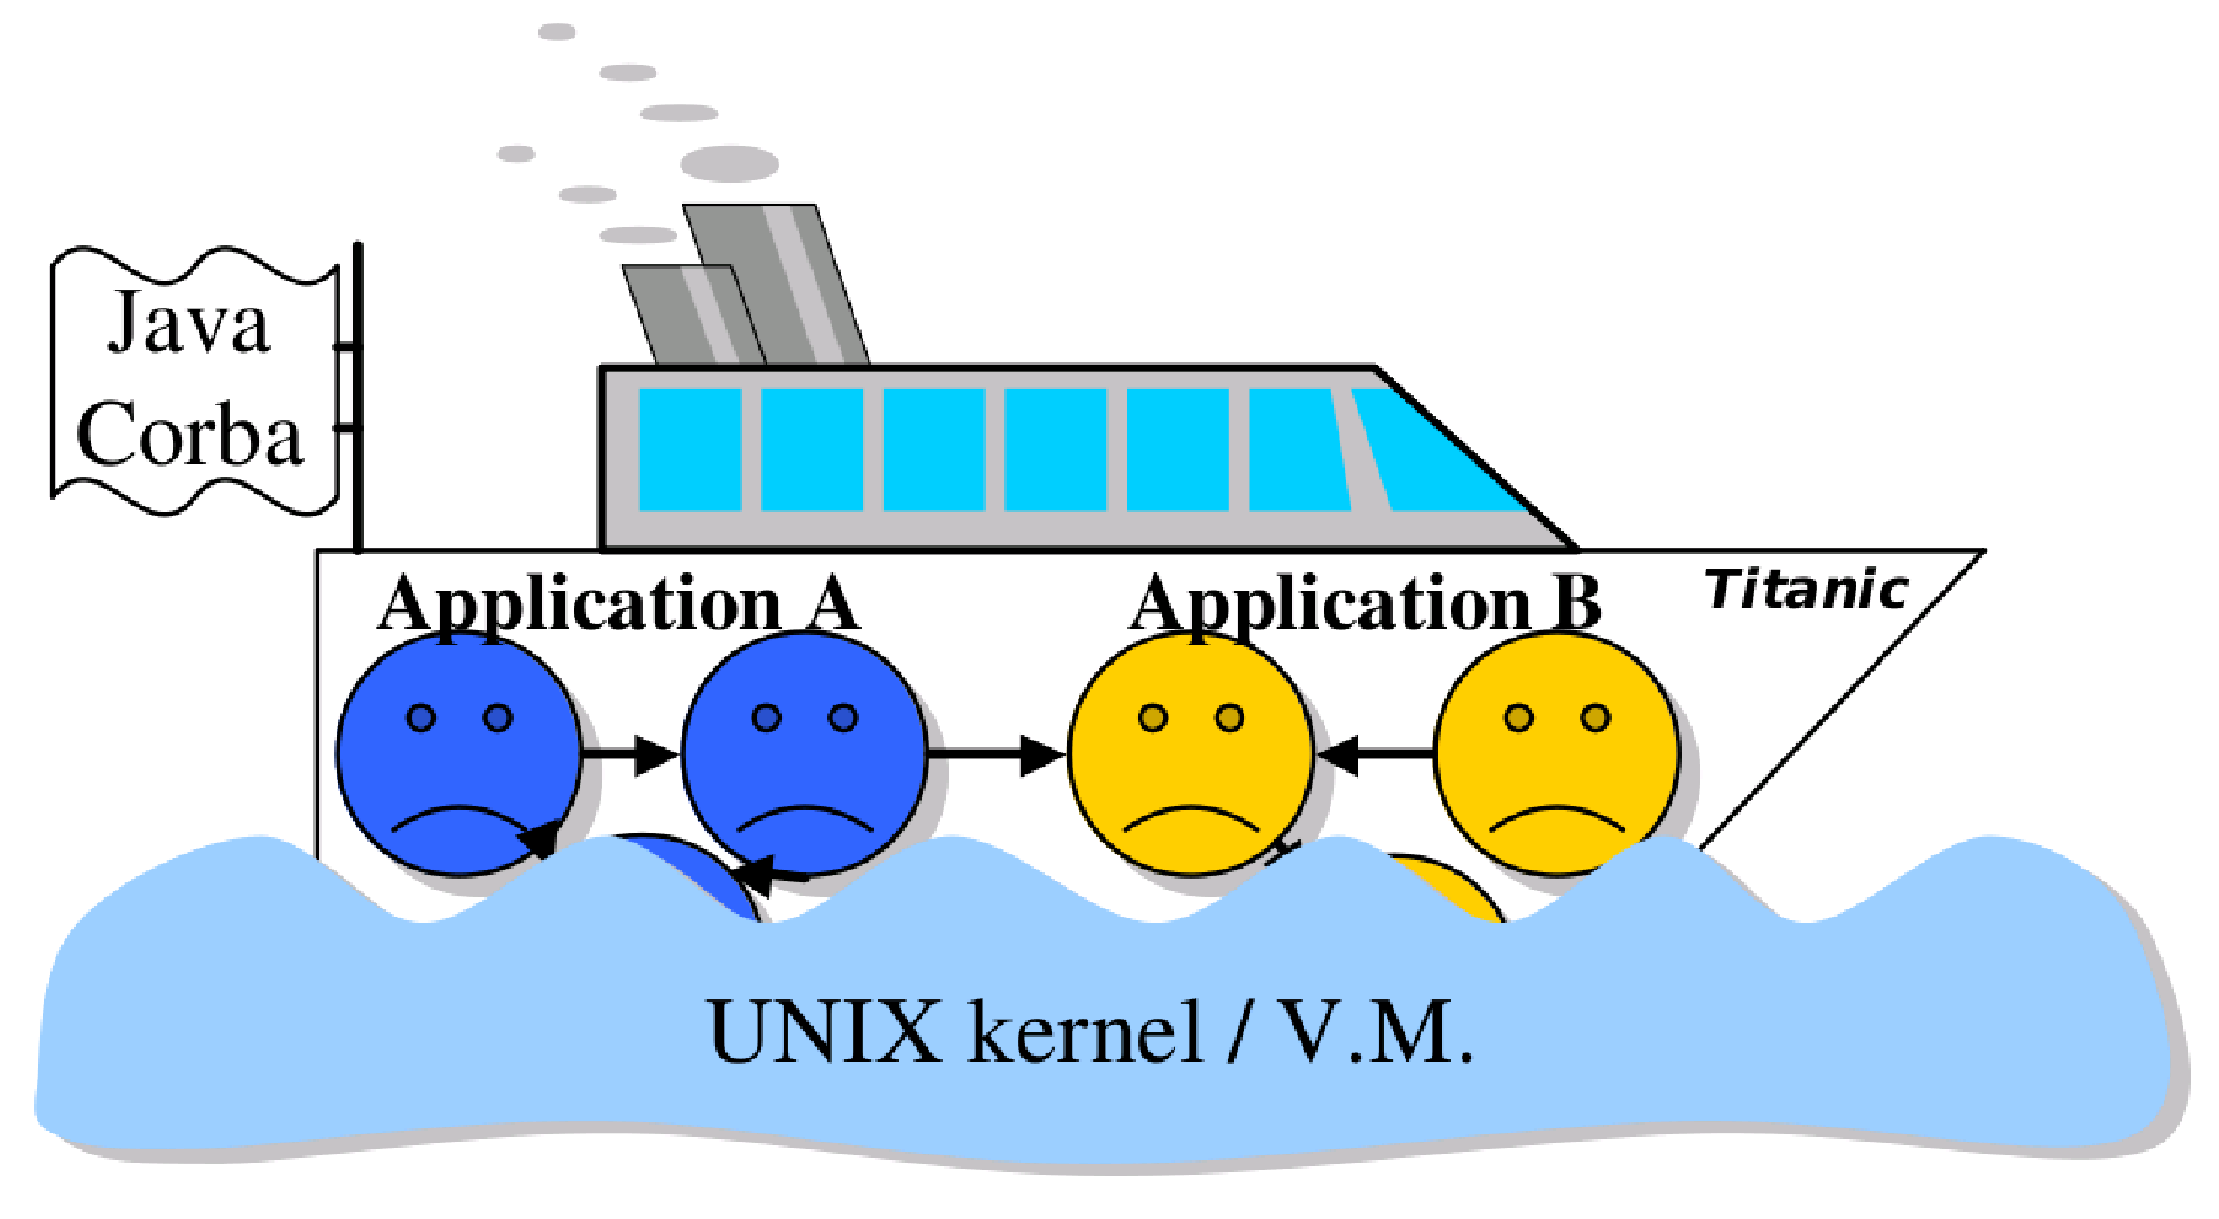
\includegraphics[scale=0.3]{figures/boat.eps}
\end{center}
\end{frame}
%---------------------------------------------------
\begin{frame}{High-level {\it{}vs} Hardware}
{\bf{}Object Oriented for Hardware}
\begin{center}
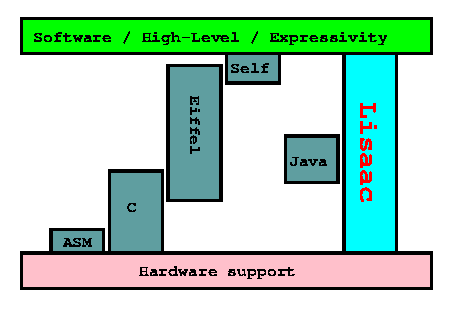
\includegraphics[scale=1.2]{figures/high_level.eps}
\end{center}
\end{frame}
%---------------------------------------------------
\begin{frame}{Class {\it{}vs} Prototype (1/3)}
\begin{block}{Class}
\begin{center}
\includegraphics[scale=1.0]{figures/class_proto.eps}
\end{center}
\end{block}
\begin{block}{Prototype}
\begin{center}
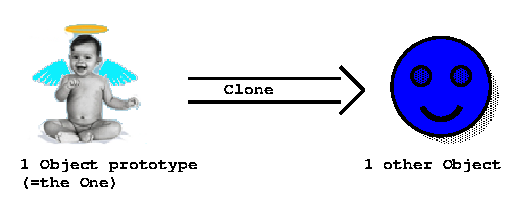
\includegraphics[scale=1.0]{figures/proto.eps}
\end{center}
\end{block}
\end{frame}
%---------------------------------------------------
\begin{frame}{Class {\it{}vs} Prototype (2/3)}
\begin{columns}
\begin{column}[l]{5.5cm}
\begin{block}{Class}
 \includegraphics[scale=0.9]{figures/herit_class.eps}
\end{block}
\end{column}
\begin{column}[r]{5.5cm}
\begin{block}{Prototype}
 \includegraphics[scale=0.9]{figures/herit_proto.eps}
\end{block}
\end{column}
\end{columns}
\end{frame}
%---------------------------------------------------
\begin{frame}{Class {\it{}vs} Prototype (3/3)}
\begin{block}{Dynamic inheritance}
\begin{center}
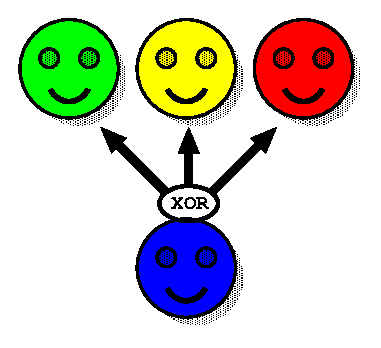
\includegraphics[scale=1.0]{figures/inherit.eps}
\end{center}
\end{block}
\end{frame}
%---------------------------------------------------
\begin{frame}{Inherit Lisaac}
\begin{itemize}
\item 
\includegraphics[scale=0.3]{figures/self.ps}
~~{\bf{}Self}\,: Flexibility, simplicity and prototype concept
\end{itemize}
\begin{center}
\textcolor{red}{$+$}
\end{center}
\begin{itemize}
\item 
\includegraphics[scale=0.3]{figures/smarteiffel.ps}
~~{\bf{}Eiffel}\,: Static type, programming by contract
\end{itemize}
\begin{center}
\textcolor{red}{$+$}
\end{center}
\begin{itemize}
\item {\bf{}C}\,: Interrupt management, memory mapping
\end{itemize}
\begin{center}
\textcolor{red}{$=$}\\

\includegraphics[scale=0.3]{figures/isaac_logo.eps}\\
~~{\bf{}Lisaac}\,: Full prototype object for hardware
\end{center}
\end{frame}
%---------------------------------------------------
\begin{frame}{Progress\ldots}
\begin{center}
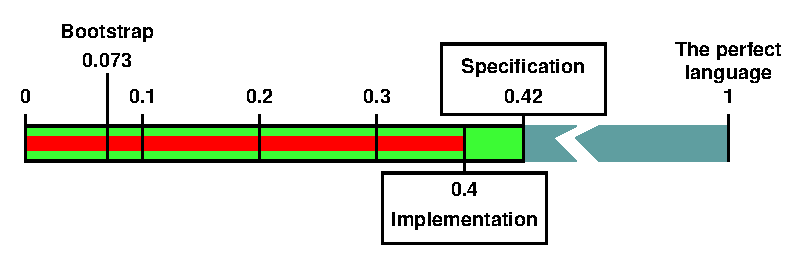
\includegraphics[scale=0.9]{figures/version.eps}
\end{center}
\end{frame}

\section{The language}
%=====================
%---------------------------------------------------
\begin{frame}{The grammar of Lisaac}
\begin{center}
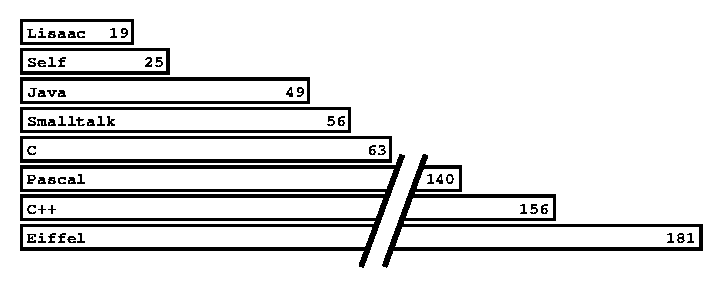
\includegraphics[scale=1.0]{figures/grammar.eps}\\
{\it{}Number of gamatical rules}
\end{center}
\end{frame}
%---------------------------------------------------
\begin{frame}{Syntax rules}
\begin{block}{Identifier}
Low case \& mono space-name environment\\
{\it{}Example\,:} \textcolor{blue}{\tt{}main, factorial}
\end{block}
\begin{block}{Keyword}
Upper case for a first character, low case else\\
{\it{}Example\,:} \textcolor{red}{\tt{}Section, Old, Private, Header}
\end{block}
\begin{block}{Type/prototype}
Upper case\\
{\it{}Example\,:} \textcolor{type}{\tt{}STRING, CHARACTER, INTEGER}
\end{block}
\begin{block}{Comment}
Like C$++$\\
{\it{}Example\,:} {\tt{}/* Comment multiline */} or {\tt{}// Comment line}
\end{block}
\end{frame}
%---------------------------------------------------
\begin{frame}{Base type (1/2)}
\begin{columns}
\begin{column}[l]{5.5cm}
\begin{block}{\textcolor{green}{\tt{}INTEGER}}
\begin{itemize}
\item {\it{}Hexadecimal\,:} \textcolor{red}{0Bh 0B80\_0000h}\\
\item {\it{}Decimal\,:} \textcolor{red}{12 12d 100\_000}\\
\item {\it{}Octal\,:} \textcolor{red}{14o 777o 7\_333o}\\
\item {\it{}Binary\,:} \textcolor{red}{01b 1101b 1010\_1111b}\\
\end{itemize}
\end{block}
\begin{block}{\textcolor{green}{\tt{}REAL}}
\begin{itemize}
\item {\it{}Simple\,:} \textcolor{red}{1.1 0.05}\\
\item {\it{}Scientific\,:} \textcolor{red}{5E-2}\\
\end{itemize}
\end{block}
\end{column}
\begin{column}[r]{5.5cm}
\begin{block}{\textcolor{green}{\tt{}CHARACTER}}
\begin{itemize}
\item {\it{}Simple\,:} \textcolor{red}{'a' 'k'}\\
\item {\it{}Escape\,:} \textcolor{red}{'$\backslash$n' '$\backslash$t'}\\
\item {\it{}Code\,:}   \textcolor{red}{'$\backslash$10$\backslash$' '$\backslash$0Ah$\backslash$'}\\
\end{itemize}
\end{block}
\begin{block}{\textcolor{green}{\tt{}STRING\_CONSTANT}}
\begin{itemize}
\item {\it{}Simple\,:} \textcolor{red}{``Hello world$\backslash$n''}\\
\item {\it{}Multiline\,:} \textcolor{red}{``Hello $\backslash$\\
$\backslash$world$\backslash$n''}\\
\end{itemize}
\end{block}
\begin{block}{\textcolor{green}{\tt{}BLOCK}}
\begin{itemize}
\item {\it{}Encapsulate code\,:} \textcolor{red}{\{ \ldots \}} {\it{}See after\ldots}\\
\end{itemize}
\end{block}
\end{column}
\end{columns}
\end{frame}
%---------------------------------------------------
\begin{frame}{Base type\,: Example (2/2)}
	
\begin{alertblock}{Warning}
Even base types are full objects!
\end{alertblock}

\begin{columns}
\begin{column}[l]{5.5cm}
\begin{block}{\textcolor{green}{\tt{}INTEGER}}
\textcolor{red}{10}\textcolor{blue}{.factorial.print};
\end{block}
\begin{block}{\textcolor{green}{\tt{}REAL}}
\textcolor{red}{2.7E-5}\textcolor{blue}{.print};
\end{block}
\end{column}
\begin{column}[r]{5.5cm}
\begin{block}{\textcolor{green}{\tt{}CHARACTER}}
\textcolor{red}{'a'}\textcolor{blue}{.to\_upper.print};
\end{block}
\begin{block}{\textcolor{green}{\tt{}STRING\_CONSTANT}}
\textcolor{red}{``Hello world$\backslash$n''}\textcolor{blue}{.print};
\end{block}
\begin{block}{\textcolor{green}{\tt{}BLOCK}}
\textcolor{red}{\{ \ldots \}}\textcolor{blue}{.value};
\end{block}
\end{column}
\end{columns}
\end{frame}
%---------------------------------------------------
\begin{frame}{Prototype}
\begin{itemize}
\item One prototype = one file 
\item The name's prototype = the name's file \\
{\it{}Example\,: }\\
The file name {\tt{}string.li} contains the \textcolor{type}{STRING} prototype.

\item One prototype is a set of \textcolor{red}{\tt{}Section}\,:
  \begin{enumerate}
  \item \textcolor{red}{\tt{}Section Header} {\it{}(Mandatory)}
  \item $n \times$ \textcolor{red}{\tt{}Section Inherit} or \textcolor{red}{\tt{}Section Insert}
  \item $n \times$ \textcolor{red}{\tt{}Section Public} or other sections\ldots
  \end{enumerate}
\item One section is a set of \textcolor{blue}{slots} {\it{}(datas or functions)}.
\end{itemize}
\end{frame}
%---------------------------------------------------
\begin{frame}{Sections}
\begin{block}{Inheritance sections after Header section}
\begin{itemize}
\item \textcolor{red}{Inherit}\,: Inheritance definition {\it{}(Private)}
\item \textcolor{red}{Insert}\,: Non-conforming inheritance {\it{}(Private)}
\end{itemize}
\end{block}
\begin{block}{Simple sections}
\begin{itemize}
\item \textcolor{red}{Public}\,: Services with public access
\item \textcolor{red}{Private}\,: Services with private access
\item \textcolor{red}{Directory}\,: Services with prototype's directory access
\item \textcolor{red}{\it{}prototype list}\,: Services with selective access
\end{itemize}
\end{block}
\begin{block}{Specific sections}
\begin{itemize}
\item \textcolor{red}{Mapping}\,: Mapping structure object
\item \textcolor{red}{Interrupt}\,: Hardware interruption handler 
\item \textcolor{red}{External}\,: External of Lisaac's slot to C function
\end{itemize}
\end{block}
\end{frame}
%---------------------------------------------------
\begin{frame}{Example\,: Hello world!}
\begin{block}{\tt{}hello.li}
\begin{alltt}
\textcolor{red}{Section Header}\\
~~\textcolor{red}{$+$} \textcolor{blue}{name} := \textcolor{type}{HELLO}; {\it{}// Mandatory}\\
\textcolor{red}{Section Public}\\
~~\textcolor{red}{$-$} \textcolor{blue}{main} $<-$ \\
~~(\\
~~~~``Hello world !$\backslash$n''.\textcolor{blue}{print};\\
~~);\\
\end{alltt}
\end{block}
{\it{}Command line\,:} {\tt{}lisaac hello.li}\\
{\it{}Executable result\,:} {\tt{}hello} {\it{}(ou {\tt{}hello.exe} for windows)}\\
\end{frame}
%---------------------------------------------------
\begin{frame}{Slot identifier}
\begin{alltt}
\textcolor{red}{$-$}\,\textcolor{blue}{qsort}\,tab:\textcolor{type}{COLLECTION}\,\textcolor{blue}{from}\,low:\textcolor{type}{INTEGER}\,\textcolor{blue}{to}\,high:\textcolor{type}{INTEGER}\,$\leftarrow$ \\
( \textcolor{red}{+} i,j:\textcolor{type}{INTEGER};\\
~~\textcolor{red}{+} x,y:\textcolor{type}{OBJECT};\\
~~i := low;\\
~~j := high;\\
~~x := tab.\textcolor{blue}{item} ((i + j)$>>$ 1);\\
~~\{ \ldots\\
~~~~(i $<=$ j).\textcolor{blue}{if} \{\\
~~~~~~tab.\textcolor{blue}{swap} j \textcolor{blue}{and} i;\\
~~~~~~\ldots\\
~~~~\};\\
~~\}.\textcolor{blue}{do\_while} \{i $<=$ j\};\\
~~(low $<$ j).\textcolor{blue}{if} \{ \textcolor{blue}{qsort} tab \textcolor{blue}{from} low \textcolor{blue}{to} j; \};\\
~~(i $<$ high).\textcolor{blue}{if} \{ \textcolor{blue}{qsort} tab \textcolor{blue}{from} i \textcolor{blue}{to} high; \};\\
);\\
\end{alltt}
\end{frame}
%---------------------------------------------------
\begin{frame}{Slot identifier}
\begin{alltt}
\textcolor{red}{$-$}\,\colorbox{red}{\textcolor{blue}{qsort}}\,tab:\textcolor{type}{COLLECTION}\,\colorbox{red}{\textcolor{blue}{from}}\,low:\textcolor{type}{INTEGER}\,\colorbox{red}{\textcolor{blue}{to}}\,high:\textcolor{type}{INTEGER}\,$\leftarrow$ \\
( \textcolor{red}{+} i,j:\textcolor{type}{INTEGER};\\
~~\textcolor{red}{+} x,y:\textcolor{type}{OBJECT};\\
~~i := low;\\
~~j := high;\\
~~x := tab.\textcolor{blue}{item} ((i + j)$>>$ 1);\\
~~\{ \ldots\\
~~~~(i $<=$ j).\textcolor{blue}{if} \{\\
~~~~~~tab.\textcolor{blue}{swap} j \textcolor{blue}{and} i;\\
~~~~~~\ldots\\
~~~~\};\\
~~\}.\textcolor{blue}{do\_while} \{i $<=$ j\};\\
~~(low $<$ j).\textcolor{blue}{if} \{ \colorbox{red}{\textcolor{blue}{qsort}} tab \colorbox{red}{\textcolor{blue}{from}} low \colorbox{red}{\textcolor{blue}{to}} j; \};\\
~~(i $<$ high).\textcolor{blue}{if} \{ \colorbox{red}{\textcolor{blue}{qsort}} tab \colorbox{red}{\textcolor{blue}{from}} i \colorbox{red}{\textcolor{blue}{to}} high; \};\\
);\\
\end{alltt}
\end{frame}
%---------------------------------------------------
\begin{frame}{Slot identifier\,: if}
\begin{alltt}
\textcolor{red}{$-$}\,\textcolor{blue}{qsort}\,tab:\textcolor{type}{COLLECTION}\,\textcolor{blue}{from}\,low:\textcolor{type}{INTEGER}\,\textcolor{blue}{to}\,high:\textcolor{type}{INTEGER}\,$\leftarrow$ \\
( \textcolor{red}{+} i,j:\textcolor{type}{INTEGER};\\
~~\textcolor{red}{+} x,y:\textcolor{type}{OBJECT};\\
~~i := low;\\
~~j := high;\\
~~x := tab.\textcolor{blue}{item} ((i + j)$>>$ 1);\\
~~\{ \ldots\\
~~~~(i $<=$ j).\colorbox{red}{\textcolor{blue}{if} \{}\\
~~~~~~tab.textcolor{blue}{swap} j \textcolor{blue}{and} i;\\
~~~~~~\ldots\\
~~~~\colorbox{red}{\}};\\
~~\}.\textcolor{blue}{do\_while} \{i $<=$ j\};\\
~~(low $<$ j).\textcolor{blue}{if} \{ \textcolor{blue}{qsort} tab \textcolor{blue}{from} low \textcolor{blue}{to} j; \};\\
~~(i $<$ high).\textcolor{blue}{if} \{ \textcolor{blue}{qsort} tab \textcolor{blue}{from} i \textcolor{blue}{to} high; \};\\
);\\
\end{alltt}
\end{frame}
%---------------------------------------------------
\begin{frame}{Slot identifier\,: loop}
\begin{alltt}
\textcolor{red}{$-$}\,\textcolor{blue}{qsort}\,tab:\textcolor{type}{COLLECTION}\,\textcolor{blue}{from}\,low:\textcolor{type}{INTEGER}\,\textcolor{blue}{to}\,high:\textcolor{type}{INTEGER}\,$\leftarrow$ \\
( \textcolor{red}{+} i,j:\textcolor{type}{INTEGER};\\
~~\textcolor{red}{+} x,y:\textcolor{type}{OBJECT};\\
~~i := low;\\
~~j := high;\\
~~x := tab.\textcolor{blue}{item} ((i + j)$>>$ 1);\\
~~\colorbox{red}{\{} \ldots\\
~~~~(i $<=$ j).\textcolor{blue}{if} \{\\
~~~~~~tab.\textcolor{blue}{swap} j \textcolor{blue}{and} i;\\
~~~~~~\ldots\\
~~~~\};\\
~~\colorbox{red}{\}.\textcolor{blue}{do\_while} \{i $<=$ j\};}\\
~~(low $<$ j).\textcolor{blue}{if} \{ \textcolor{blue}{qsort} tab \textcolor{blue}{from} low \textcolor{blue}{to} j; \};\\
~~(i $<$ high).\textcolor{blue}{if} \{ \textcolor{blue}{qsort} tab \textcolor{blue}{from} i \textcolor{blue}{to} high; \};\\
);\\
\end{alltt}
\end{frame}
%---------------------------------------------------
\begin{frame}{Arguments/results definition}
\begin{block}{Argument}
\begin{itemize}
\item Simple\,: {\tt{}\textcolor{blue}{qsort} tab:\textcolor{type}{COLLECTION}}
\item Vector\,: {\tt{}\textcolor{blue}{put\_pixel} (x,y:\textcolor{type}{INTEGER})}
\end{itemize}
\end{block}
\begin{block}{Result}
\begin{itemize}
\item Simple\,: {\tt{}\textcolor{blue}{is\_even}:\textcolor{type}{BOOLEAN}}
\item Vector\,: {\tt{}\textcolor{blue}{get\_coord}:(\textcolor{type}{INTEGER,INTEGER})}
\end{itemize}
\end{block}
\end{frame}
%---------------------------------------------------
\begin{frame}{Operator slot\,: Unary (1/3)}
\begin{block}{Prefix}
\begin{alltt}
\textcolor{red}{-} \textcolor{blue}{'-'} Self:\textcolor{type}{SELF} :\textcolor{type}{SELF} $\leftarrow$\\
\textcolor{blue}{zero} - Self; {\it{}// Self $\equiv$ this}
\end{alltt}
{\it{}Example\,:} {\tt{}(-3).\textcolor{blue}{print};}
\end{block}
\begin{block}{Postfix}
\begin{alltt}
\textcolor{red}{-} Self:\textcolor{type}{SELF} \textcolor{blue}{'!'} :\textcolor{type}{SELF} $\leftarrow$\\
( \textcolor{red}{+} result:\textcolor{type}{INTEGER};\\
~~(Self = 0).\textcolor{blue}{if}~~ \{ result := 1; ~~~~~~~~~~~\} \\
~~~~~~~~~~~~~\textcolor{blue}{else} \{ result := (Self - 1) \textcolor{blue}{!}; \};\\
~~result\\
);
\end{alltt}
{\it{}Example\,:} {\tt{}(10 !).\textcolor{blue}{print};};
\end{block}
\end{frame}
%---------------------------------------------------
\begin{frame}{Operator slot\,: Binary (2/3)}
\begin{block}{Infix associativity {\bf{}left} priority {\bf{}80}}
\begin{alltt}
\textcolor{red}{-} Self:\textcolor{type}{SELF} \textcolor{blue}{'+'} \textcolor{red}{Left 80} other:\textcolor{type}{SELF} :\textcolor{type}{SELF} $\leftarrow$\\
Self - - other;
\end{alltt}
{\it{}Example\,:} {\tt{}2 + 3 + 4 = ((2 + 3) + 4)}
\end{block}

\begin{block}{Infix associativity {\bf{}left} priority {\bf{}90}}
\begin{alltt}
\textcolor{red}{-} Self:\textcolor{type}{SELF} \textcolor{blue}{'*'} \textcolor{red}{Left 90} other:\textcolor{type}{SELF} :\textcolor{type}{SELF} $\leftarrow$ \ldots
\end{alltt}
{\it{}Example\,:} {\tt{}2 + 3 * 4 = (2 + (3 * 4))}
\end{block}
\begin{block}{Infix associativity {\bf{}right} priority {\bf{}90}}
\begin{alltt}
\textcolor{red}{-} Self:\textcolor{type}{SELF} \textcolor{blue}{'$\wedge$'} \textcolor{red}{right 90} other:\textcolor{type}{SELF} :\textcolor{type}{SELF} $\leftarrow$ \ldots
\end{alltt}
{\it{}Example\,:} {\tt{}2 $\wedge$ 3 $\wedge$ 4 = (2 $\wedge$ (3 $\wedge$ 4))}
\end{block}
\end{frame}
%---------------------------------------------------
\begin{frame}{Operator slot (3/3)}
\begin{alertblock}{Priority}
\begin{enumerate}
\item Classic message\\
{\it{}Example\,:} {\tt{}2 + 5.factorial} $\Longleftrightarrow$ {\tt{}2 + (5.factorial)}
\item Postfix message\\
{\it{}Example\,:} {\tt{}- 5 !} $\Longleftrightarrow$ {\tt{}- (5 !)}
\item Prefix message\\
{\it{}Example\,:} {\tt{}2 + - 5} $\Longleftrightarrow$ {\tt{}2 + (- 5)}
\item Infix message\: Depending priority\\
{\it{}Example\,:} {\tt{}2 + 3 * 5} $\Longleftrightarrow$ {\tt{}2 + (3 * 5)}
\end{enumerate}
\end{alertblock}
\begin{block}{Character list for operator {\it{}(It's free style!)}}
\begin{alltt}
!~~@~~\#~~\$~~\%~~$\wedge$~~\&~~$<$~~| ~~~~~\textcolor{red}{(<-~~?= impossible)}\\
*~~+~~-~~=~~$\sim$~~/~~?~~$>$~~$\backslash$
\end{alltt}
\end{block}
\end{frame}
%---------------------------------------------------
\begin{frame}{Style slot (1/3)}
\begin{block}{\textcolor{red}{+}\,: No shared, clonable or call sensitif}
\begin{itemize}
\item Distinct for classic data slot
\item Distinct for classic local slot (Local variable)
\end{itemize}
\end{block}
\begin{block}{\textcolor{red}{$-$}\,: Shared (= \textcolor{red}{{\tt{}static}} in java), persistant value}
\begin{itemize}
\item For method slot
\item For static data slot or local
\end{itemize}
\end{block}
\end{frame}
%---------------------------------------------------
\begin{frame}{Style slot (2/3)}
\begin{block}{No shared {\it{}vs} shared}
\begin{center}
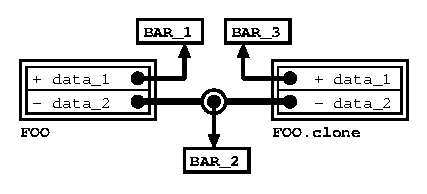
\includegraphics[scale=1.5]{figures/expanded_general.eps}
\end{center}
\end{block}
\end{frame}
%---------------------------------------------------
\begin{frame}{Style slot (3/3)}
\begin{columns}
\begin{column}[l]{5.5cm}
\begin{block}{Step \#0}
\includegraphics[scale=0.75]{figures/style.eps}
\end{block}
\begin{block}{Step \#3}
\begin{alltt}
\textcolor{blue}{foo2.set\_data\_1} \textcolor{type}{BAR\_3};\\
\textcolor{blue}{foo2.set\_data\_2} \textcolor{type}{BAR\_4};\\
\end{alltt}
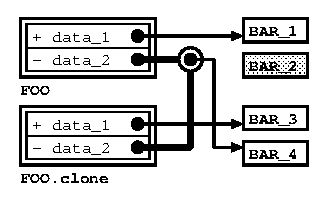
\includegraphics[scale=0.75]{figures/style4.eps}
\end{block}
\end{column}

\begin{column}[r]{5.5cm}
\begin{block}{Step \#1}
\begin{alltt}
\textcolor{blue}{data\_1} := \textcolor{type}{BAR\_1};\\
\textcolor{blue}{data\_2} := \textcolor{type}{BAR\_2};\\
\end{alltt}
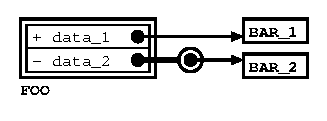
\includegraphics[scale=0.75]{figures/style2.eps}
\end{block}
\begin{block}{Step \#2}
\begin{alltt}
\textcolor{blue}{foo2} := \textcolor{type}{FOO}.\textcolor{blue}{clone};\\
\end{alltt}
\includegraphics[scale=0.75]{figures/style3.eps}
\end{block}
\end{column}
\end{columns}
\end{frame}
%---------------------------------------------------
\begin{frame}{Expanded attribute = Embedded object (1/2)}
\begin{block}{Default attribute (in header declaration)}
\begin{columns}
\begin{column}[l]{6cm}
\begin{alltt}
\textcolor{red}{Section Header}\\
~~\textcolor{red}{$+$} \textcolor{blue}{name} := \textcolor{red}{Expanded} \textcolor{type}{INTEGER};\\
\end{alltt}
\end{column}
\begin{column}[r]{3cm}
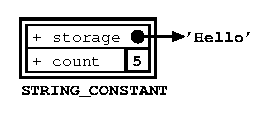
\includegraphics[scale=0.75]{figures/expanded1.eps}
\end{column}
\end{columns}
{\it{}Examples\,:} All tiny objects like \textcolor{type}{{\tt{}CHARACTER, REALs, INTEGERs}}
\end{block}
\begin{block}{Attribute type declaration}
\begin{columns}
\begin{column}[l]{5cm}
\begin{alltt}
\textcolor{red}{$+$} \textcolor{blue}{slot}:\textcolor{type}{STRING\_CONSTANT};\\
\end{alltt}
\end{column}
\begin{column}[r]{5cm}
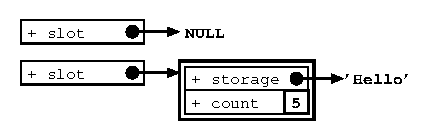
\includegraphics[scale=0.75]{figures/expanded2.eps}
\end{column}
\end{columns}
\begin{alltt}
\textcolor{red}{$+$} \textcolor{blue}{slot}:\textcolor{red}{Expanded} \textcolor{type}{STRING\_CONSTANT};\\
\end{alltt}
\begin{columns}
\begin{column}[l]{5cm}
\includegraphics[scale=0.75]{figures/expanded3.eps}
\end{column}
\begin{column}[r]{5cm}
\textcolor{red}{{\tt{}Expanded} slot is never NULL!}
\end{column}
\end{columns}
\end{block}
\end{frame}
%---------------------------------------------------
\begin{frame}{Expanded attribute \& inheritance (2/2)}
\begin{alertblock}{Definition}
\begin{center}
Distinct \& Expanded inheritance slot\\
$\Longleftrightarrow$\\
Class inheritance system (= Java like)
\end{center}
\begin{alltt}
\textcolor{red}{Section Header}\\
~~\textcolor{red}{$+$} \textcolor{blue}{name} := \textcolor{type}{DOG};\\
\textcolor{red}{Section Inherit}\\
~~\textcolor{red}{$+$} \textcolor{blue}{parent\_animal}:\textcolor{red}{Expanded} \textcolor{type}{ANIMAL};\\
\end{alltt}
\end{alertblock}
\begin{exampleblock}{Note}
All other inheritance slot combinations $\Longrightarrow$ Prototype system only
\end{exampleblock}
\end{frame}
%---------------------------------------------------
\begin{frame}{Strict attribute}
\begin{block}{Strict\,: Static type $\Longrightarrow$ dynamic type}
\begin{alltt}
~~\textcolor{red}{$+$} \textcolor{blue}{data}:\textcolor{red}{Strict} \textcolor{type}{FRUIT};\\
\ldots\\
~~\textcolor{blue}{data} := \textcolor{type}{APPLE}.\textcolor{blue}{clone}; // \textcolor{red}{IMPOSSIBLE!!!}\\
~~\textcolor{blue}{data} := \textcolor{type}{FRUIT}.\textcolor{blue}{clone}; // \textcolor{red}{OK!}\\
\end{alltt}
\end{block}
\begin{exampleblock}{Note}
{\tt{}Expanded} attribute $\Longrightarrow$ {\tt{}Strict} attribut
\end{exampleblock}
\end{frame}
%---------------------------------------------------
\begin{frame}{SELF type}
\begin{block}{SELF\,: Dynamic type $\Longrightarrow$ static type}
In \textcolor{type}{FRUIT}\,:
\begin{alltt}
~~\textcolor{red}{$-$} \textcolor{blue}{clone}:\textcolor{type}{SELF} $\leftarrow$ \ldots\\
\end{alltt}
With \textcolor{type}{APPLE} and \textcolor{type}{ORANGE} inherit \textcolor{type}{FRUIT}\,:
\begin{alltt}
apple  := \textcolor{type}{APPLE}.\textcolor{blue}{clone}; // \textcolor{red}{return Strict APPLE}\\
orange := \textcolor{type}{ORANGE}.\textcolor{blue}{clone}; // \textcolor{red}{return Strict ORANGE}\\
\end{alltt}
\end{block}
\begin{exampleblock}{Note}
\begin{itemize}
\item Self type $\Longrightarrow$ {\tt{}Strict} attribute
\item {\bf{}Data slot} or {\bf{}shared local} variable with SELF type is impossible!
\end{itemize}
\end{exampleblock}
\end{frame}
%---------------------------------------------------
\begin{frame}{Genericity type}

\begin{block}{Declaration in header}
\begin{alltt}
\textcolor{red}{Section Header}\\
~~\textcolor{red}{$+$} \textcolor{blue}{name} := \textcolor{type}{ARRAY(E)};\\
\end{alltt}
\end{block}

\begin{exampleblock}{Note}
\textcolor{type}{E} is parameter type. Syntax\,: $[A..Z][0..9]^*$
\end{exampleblock}

\begin{block}{Example}
\begin{alltt}
~~\textcolor{red}{$+$} bucket:\textcolor{type}{ARRAY(FRUIT)};\\
~~bucket := \textcolor{type}{ARRAY(FRUIT)}.\textcolor{blue}{create} 2;\\
~~bucket.\textcolor{blue}{put} \textcolor{type}{ORANGE} \textcolor{blue}{to} 1;\\
~~bucket.\textcolor{blue}{put} \textcolor{type}{APPLE} \textcolor{blue}{to} 2;
\end{alltt}
\end{block}
\end{frame}
%---------------------------------------------------
\begin{frame}{Parameters' types used in the method (without genericity)}
\begin{block}{Example}
\begin{alltt}
~~\textcolor{red}{$-$} \textcolor{blue}{max} a:\textcolor{type}{E} \textcolor{blue}{and} b:\textcolor{type}{E} :\textcolor{type}{E} $\leftarrow$ \\
~~( \textcolor{red}{$+$} result:\textcolor{type}{E};\\
~~~~(a > b).\textcolor{blue}{if} \{\\
~~~~~~result := a;\\
~~~~\} \textcolor{blue}{else} \{\\
~~~~~~result := b;\\
~~~~\};\\
~~~~result\\
~~);\\
\end{alltt}
\end{block}
\begin{exampleblock}{Note}
All parameter type must be defined in arguments function.
\end{exampleblock}
\end{frame}
%---------------------------------------------------
\begin{frame}{Same prototype name}
\begin{block}{Example}
\begin{alltt}
\textcolor{type}{DIRECTORY.FOO}.\textcolor{blue}{message}; \\
\textcolor{type}{DIRECTORY1.DIRECTORY2.DIRECTORY3.FOO} \\
\textcolor{type}{DIRECTORY1...FOO} \\
\end{alltt}
\end{block}
\begin{center}
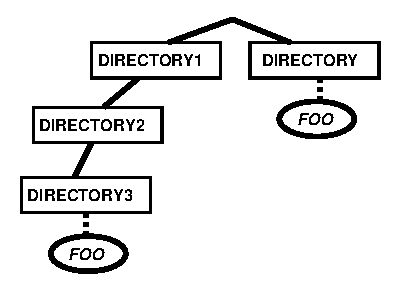
\includegraphics[scale=0.95]{figures/directory.eps}
\end{center}
\end{frame}
%---------------------------------------------------
\begin{frame}{Assignment\,: data (1/3)}
\begin{block}{Example}
\begin{alltt}
~~( \textcolor{red}{$+$} f:\textcolor{type}{FRUIT};\\
~~~~\textcolor{red}{$+$} a:\textcolor{type}{APPLE};\\
~~~~a := \textcolor{type}{APPLE};\\
~~~~f := a;\\
~~);\\
\end{alltt}
\end{block}
\begin{exampleblock}{Note}
\begin{itemize}
\item Assignment is statically ok, if the static type is an identical or a sub-type.
\item Simple data assignment ':=' is the '=' in Java, C$++$, \ldots
\item Warning with {\bf{}Strict attribute} type {\it{}(see before \ldots)}
\end{itemize}
\end{exampleblock}
\end{frame}
%---------------------------------------------------
\begin{frame}{Assignment\,: data, if possible (2/3)}
\begin{block}{Example}
\begin{alltt}
~~( \textcolor{red}{$+$} f:\textcolor{type}{FRUIT};\\
~~~~\textcolor{red}{$+$} a:\textcolor{type}{APPLE};\\
~~~~(test).\textcolor{blue}{if} \{\\
~~~~~~f := \textcolor{type}{APPLE};\\
~~~~\} \textcolor{blue}{else} \{\\
~~~~~~f := \textcolor{type}{ORANGE};\\
~~~~\};\\
~~~~a ?= f;  // \textcolor{red}{a=f, if f is APPLE, a=NULL else}\\
~~);\\
\end{alltt}
\end{block}
\begin{exampleblock}{Note}
\begin{itemize}
\item Assignment is dynamically ok, if the dynamic type is identical or sub-type.
\item This mechanism replaces the cast of Java
\end{itemize}
\end{exampleblock}
\end{frame}
%---------------------------------------------------
\begin{frame}{Assignment\,: code (3/3)}
\begin{block}{Example}
\begin{columns}
\begin{column}[l]{6cm}
\begin{alltt}
\textcolor{red}{$-$} \textcolor{blue}{color} (r,g,b:\textcolor{type}{INTEGER}) $<-$ \\
( \\
~~\textcolor{blue}{true\_color}:=r$<<$16|g$<<$8|b;\\
);\\
\ldots\\
( \\
~~\textcolor{blue}{color} $<-$ (\\
~~~~\textcolor{blue}{gray\_color} := (r+g+b)/3;\\
~~);\\
);\\
\end{alltt}
\end{column}
\begin{column}[r]{4cm}
\includegraphics[scale=0.175]{figures/flower.ps}
\end{column}
\end{columns}
\end{block}
\end{frame}
%---------------------------------------------------
\begin{frame}{Inheritance\,: Class like (1/6)}
\begin{block}{\textcolor{red}{$+$} \& \textcolor{red}{Expanded} = Class system}
\begin{alltt}
\textcolor{red}{Section Inherit}\\
~~\textcolor{red}{$+$} \textcolor{blue}{parent\_animal}:\textcolor{red}{Expanded} \textcolor{type}{ANIMAL};\\
\end{alltt}
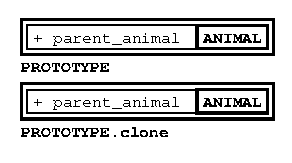
\includegraphics[scale=1.0]{figures/inherit1.eps}
\end{block}
\end{frame}
%---------------------------------------------------
\begin{frame}{Inheritance\,: Prototype ``trait'' {\it{}(Self like)} (2/6)}
\begin{block}{\textcolor{red}{$-$} = Full shared}
\begin{alltt}
\textcolor{red}{Section Inherit}\\
~~\textcolor{red}{$-$} \textcolor{blue}{parent\_object}:\textcolor{type}{OBJECT} := \textcolor{type}{OBJECT};\\
\end{alltt}
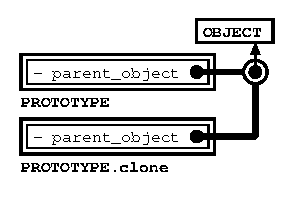
\includegraphics[scale=1.0]{figures/inherit2.eps}
\end{block}
\end{frame}
%---------------------------------------------------
\begin{frame}{Inheritance\,: No shared \& dynamic {\it{}(Lisaac inside)} (3/6)}
\begin{block}{\textcolor{red}{$+$} = Full dynamic}
\begin{alltt}
\textcolor{red}{Section Inherit}\\
~~\textcolor{red}{$+$} \textcolor{blue}{parent\_object}:\textcolor{type}{OBJECT} := \textcolor{type}{OBJECT};\\
\textcolor{red}{Section Public}\\
\ldots\\
~~~~\textcolor{blue}{parent\_object} := \textcolor{type}{FILE};\\
\ldots\\
~~~~\textcolor{blue}{parent\_object} := \textcolor{type}{DIRECTORY};\\
\end{alltt}
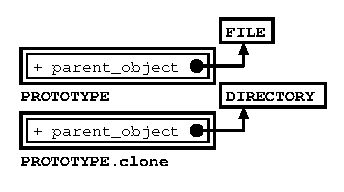
\includegraphics[scale=1.0]{figures/inherit3.eps}
\end{block}
\end{frame}
%---------------------------------------------------
\begin{frame}{Inheritance\,: Shared \& Embedded {\it{}(Lisaac inside)} (4/6)}
\begin{block}{\textcolor{red}{$-$} \& \textcolor{red}{Expanded} {\it{}(uniformity form)}}
\begin{alltt}
\textcolor{red}{Section Inherit}\\
~~\textcolor{red}{$-$} \textcolor{blue}{parent\_object}:\textcolor{red}{Expanded} \textcolor{type}{OBJECT};\\
\end{alltt}
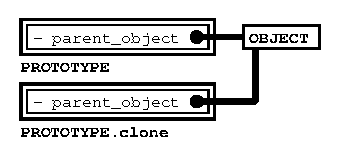
\includegraphics[scale=1.0]{figures/inherit4.eps}
\end{block}
\end{frame}
%---------------------------------------------------
\begin{frame}{Inheritance\,: Dynamic compute parent {\it{}(Lisaac inside)} (5/6)}
\begin{block}{For each lookup}
\begin{alltt}
\textcolor{red}{Section Inherit}\\
~~\textcolor{red}{$+$} \textcolor{blue}{parent}:\textcolor{type}{OBJECT} $\leftarrow$\\
~~( \textcolor{red}{$+$} result:\textcolor{type}{OBJECT};\\
~~~~\ldots  // {\it{} compute my parent}\\
~~~~result\\
~~);\\
\end{alltt}
\end{block}
\begin{alertblock}{Warning}
Endless Recursivity caused by the lookup algorithm.
\end{alertblock}
\end{frame}
%---------------------------------------------------
\begin{frame}{Inheritance\,: Dynamic once compute parent {\it{}(Lisaac inside)} (6/6)}
\begin{block}{Once execution dynamic parent evaluation}
\begin{alltt}
\textcolor{red}{Section Inherit}\\
~~\textcolor{red}{$+$} \textcolor{blue}{parent}:\textcolor{type}{OBJECT} $\leftarrow$\\
~~( \textcolor{red}{$+$} result:\textcolor{type}{OBJECT};\\
~~~~\ldots  // {\it{} compute my parent}\\
~~~~\textcolor{blue}{parent} := result  // {\it{}my parent is a data now!!!}\\
~~);\\
\end{alltt}
\end{block}
\begin{exampleblock}{Note}
\begin{itemize}
\item The first lookup, the parent is dynamically defined
\item The next lookup, the parent is a simple data value
\end{itemize}
\end{exampleblock}
\end{frame}
%---------------------------------------------------
\begin{frame}{Non-conforming inheritance}
\begin{block}{\textcolor{red}{Insert} keyword}
\begin{columns}
\begin{column}[l]{7cm}
\begin{alltt}
\textcolor{red}{Section Header}\\
~~\textcolor{red}{$+$} \textcolor{blue}{name} := \textcolor{type}{HUMAN};\\
\textcolor{red}{Section Insert}\\
~~\textcolor{red}{$+$} \textcolor{blue}{parent\_mammal}:\textcolor{red}{Expanded} \textcolor{type}{MAMMAL};\\
\end{alltt}
\end{column}
\begin{column}[r]{2cm}

\includegraphics[scale=1.0]{figures/human.eps}
\end{column}
\end{columns}
\end{block}
\begin{block}{Example}
\begin{alltt}
~~\textcolor{red}{$+$} a:\textcolor{type}{MAMMAL};\\
~~a := \textcolor{type}{HUMAN}.\textcolor{blue}{clone}; // \textcolor{red}{Impossible!!!}\\
\end{alltt}

\end{block}
\begin{alertblock}{Warning}
The \textcolor{red}{Expanded} default object has always non-conforming inheritance
\end{alertblock}
\end{frame}
%---------------------------------------------------
\begin{frame}{List\,: Set of Instructions \& immediate evaluation (1/3)}
\begin{columns}
\begin{column}[l]{5cm}
\begin{block}{Without return value}
\begin{alltt}
\textcolor{red}{(} $< Local >$;\\
~~$< Expr 1>$;\\
~~$< Expr 2>$;\\
~~$< Expr 3>$;\\
\textcolor{red}{)}
\end{alltt}
\end{block}

\begin{block}{With one return value}
\begin{alltt}
\textcolor{red}{(} $< Local >$;\\
~~$< Expr 1>$;\\
~~$< Expr 2>$;\\
~~$< result>$\\
\textcolor{red}{)}
\end{alltt}
\end{block}
\end{column}
\begin{column}[r]{5cm}
\begin{block}{With $n$ return value}
\begin{alltt}
\textcolor{red}{(} $< Local >$;\\
~~$< Expr 1>$;\\
~~$< Expr 2>$;\\
~~$< result1>$,\\
~~$< result2>$\\
\textcolor{red}{)}
\end{alltt}
\end{block}
\end{column}
\end{columns}
\end{frame}
%---------------------------------------------------
\begin{frame}{List\,: Examples (2/3)}
\begin{block}{For expressions}
\begin{alltt}
\textcolor{red}{(}2 + 4\textcolor{red}{)} * 7
\end{alltt}
\end{block}
\begin{block}{For procedures}
\begin{alltt}
\textcolor{red}{-} \textcolor{blue}{foo} $\leftarrow$\\
\textcolor{red}{(}\\
~~''Hello''.\textcolor{blue}{print};\\
\textcolor{red}{)};
\end{alltt}
\end{block}
\begin{block}{For functions}
\begin{alltt}
\textcolor{red}{-} \textcolor{blue}{zero}:\textcolor{type}{INTEGER} $\leftarrow$\\
\textcolor{red}{(}\\
~~''Call zero''.\textcolor{blue}{print};\\
~~0\\
\textcolor{red}{)};
\end{alltt}
\end{block}
\end{frame}
%---------------------------------------------------
\begin{frame}{List\,: Examples (3/3)}
\begin{block}{For vector assignment}
\begin{alltt}
\textcolor{red}{(}a,b\textcolor{red}{)} := \textcolor{red}{(}3,7\textcolor{red}{)};
\end{alltt}
\end{block}
\begin{block}{For functions with resultS}
\begin{alltt}
\textcolor{red}{-} \textcolor{blue}{coord}:\textcolor{red}{(}\textcolor{type}{INTEGER,INTEGER}\textcolor{red}{)} $\leftarrow$
\textcolor{red}{(} \textcolor{blue}{x\_current,y\_current} \textcolor{red}{)};
\end{alltt}
\end{block}
\begin{block}{For vector argument}
\begin{alltt}
\textcolor{blue}{put\_pixel} \textcolor{red}{(}x,y\textcolor{red}{)} \textcolor{blue}{color} 0;
\end{alltt}
\end{block}
\begin{block}{Plugin of vectors}
\begin{alltt}
\textcolor{red}{(}x,y\textcolor{red}{)} := \textcolor{blue}{get\_coord};\\
\textcolor{blue}{put\_pixel} \textcolor{red}{(}x,y\textcolor{red}{)} \textcolor{blue}{color} 0;\\
~~~~~~~~~~\textcolor{red}{$\equiv$}\\
\textcolor{blue}{put\_pixel} \textcolor{blue}{get\_coord} \textcolor{blue}{color} 0;
\end{alltt}
\end{block}
\end{frame}
%---------------------------------------------------
\begin{frame}{\textcolor{green}{BLOCK}\,: Set of instructions \& late evaluation (1/4)}
\begin{columns}
\begin{column}[l]{5cm}
\begin{block}{Without return value}
\begin{alltt}
\textcolor{red}{\{} $< Args >$;\\
~~$< Local >$;\\
~~$< Expr 1>$;\\
~~$< Expr 2>$;\\
\textcolor{red}{\}}
\end{alltt}
\end{block}

\begin{block}{With one return value}
\begin{alltt}
\textcolor{red}{\{} $< Args >$;\\
~~$< Local >$;\\
~~$< Expr 1>$;\\
~~$< Expr 2>$;\\
~~$< result>$\\
\textcolor{red}{\}}
\end{alltt}
\end{block}
\end{column}
\begin{column}[r]{5cm}
\begin{block}{With $n$ return value}
\begin{alltt}
\textcolor{red}{\{} $< Args >$;\\
~~$< Local >$;\\
~~$< Expr 1>$;\\
~~$< Expr 2>$;\\
~~$< result1>$,\\
~~$< result2>$\\
\textcolor{red}{\}}
\end{alltt}
\end{block}
\end{column}
\end{columns}
\end{frame}
%---------------------------------------------------
\begin{frame}{\textcolor{green}{BLOCK} {\it{}vs} List (2/4)}
\begin{block}{List}
\begin{alltt}
\textcolor{red}{(} $< Local >$;\\
~~$< Expr 1>$;\\
~~$< Expr 2>$;\\
~~$< Expr 3>$;\\
\textcolor{red}{)}
\end{alltt}
\end{block}
\begin{center}
\textcolor{red}{{\bf{}$\equiv$}}
\end{center}
\begin{block}{\textcolor{green}{BLOCK}.value}
\begin{alltt}
\textcolor{red}{\{} $< Local >$;\\
~~$< Expr 1>$;\\
~~$< Expr 2>$;\\
~~$< Expr 3>$;\\
\textcolor{red}{\}}.\textcolor{blue}{value}
\end{alltt}
\end{block}
\end{frame}
%---------------------------------------------------
\begin{frame}{\textcolor{green}{BLOCK}\,: Example (3/4)}
\begin{block}{Embedded code in object}
\begin{alltt}
\textcolor{red}{+} display:\textcolor{type}{\{(INTEGER,INTEGER); INTEGER\}};\\
display := \textcolor{red}{\{} (x,y:\textcolor{type}{INTEGER});  // {\it{}Vector parameter}\\
~~~~~~~~~~~~~\textcolor{red}{+} sum:\textcolor{type}{INTEGER};  // {\it{}One local variable}\\
~~~~~~~~~~~~~x.\textcolor{blue}{print};\\
~~~~~~~~~~~~~','.\textcolor{blue}{print};\\
~~~~~~~~~~~~~y.\textcolor{blue}{print};\\
~~~~~~~~~~~~~sum := x + y;\\
~~~~~~~~~~~~~sum  // {\it{}The result block}\\
~~~~~~~~~~~\textcolor{red}{\}};\\
\ldots\\
display.\textcolor{blue}{value} (3,4) .\textcolor{blue}{print};
\end{alltt}
\end{block}
\end{frame}
%---------------------------------------------------
\begin{frame}{\textcolor{green}{BLOCK}\,: Examples (4/4)}
\begin{block}{For expressions}
\begin{alltt}
(a != \textcolor{type}{NULL}) \&\& \textcolor{red}{\{}a.\textcolor{blue}{value} = 3\textcolor{red}{\}}
\end{alltt}
\end{block}
\begin{block}{For conditionals}
\begin{alltt}
(a > b).\textcolor{blue}{if} \textcolor{red}{\{} \\
~~'y'.\textcolor{blue}{print};\\
\textcolor{red}{\}} \textcolor{blue}{else} \textcolor{red}{\{}\\
~~'n'.\textcolor{blue}{print};\\
\textcolor{red}{\}};
\end{alltt}
\end{block}
\begin{columns}
\begin{column}[l]{5cm}
\begin{block}{For loops}
\begin{alltt}
\textcolor{red}{\{} j := j + 1;\\
~~j.\textcolor{blue}{print};\\
\textcolor{red}{\}}.\textcolor{blue}{do\_while} \textcolor{red}{\{}j < 10\textcolor{red}{\}};
\end{alltt}
\end{block}
\end{column}
\begin{column}[r]{5cm}
\begin{block}{For iterations}
\begin{alltt}
1.\textcolor{blue}{to} 10 \textcolor{blue}{do} \textcolor{red}{\{} j:\textcolor{type}{INTEGER};\\
~~j.\textcolor{blue}{print};\\
\textcolor{red}{\}};
\end{alltt}
\end{block}
\end{column}
\end{columns}
\end{frame}
%---------------------------------------------------
\begin{frame}{C like Switch statement (1/3)}
\begin{block}{For vector assignment}
\begin{alltt}
foo.\textcolor{blue}{switch}\\
.\textcolor{blue}{case} 1 \textcolor{blue}{do} \textcolor{red}{\{}\\
~~``Case 1''.\textcolor{blue}{print};  \\
\textcolor{red}{\}}.\textcolor{blue}{break}\\
.\textcolor{blue}{case} 2 \textcolor{blue}{do} \textcolor{red}{\{}\\
~~``Case 2''.\textcolor{blue}{print};\\
\textcolor{red}{\}}\\
.\textcolor{blue}{case} 3 \textcolor{blue}{do} \textcolor{red}{\{}\\
~~``Case 3''.\textcolor{blue}{print};\\
\textcolor{red}{\}}\\
.\textcolor{blue}{default} \textcolor{red}{\{}\\
~~``Default case''.\textcolor{blue}{print};\\
\textcolor{red}{\}};
\end{alltt}
\end{block}
\end{frame}
%---------------------------------------------------
\begin{frame}{C like Switch statement (2/3)}
\begin{alltt}
\textcolor{red}{-} Self:\textcolor{type}{SELF}.\textcolor{blue}{switch}:(\textcolor{type}{SELF,INTEGER\_8}) <- (Self, 0);\\

\textcolor{red}{-} (Self:\textcolor{type}{SELF}, stat:\textcolor{type}{INTEGER\_8}).\textcolor{blue}{case}\\
~~value:\textcolor{type}{SELF} \textcolor{blue}{do} body:\textcolor{red}{\{\}} :(\textcolor{type}{SELF,INTEGER\_8}) <-\\ 
( \textcolor{red}{+} new\_stat:\textcolor{type}{INTEGER\_8};\\
~~Self, \\
~~(((stat = 0) \&\& \textcolor{red}{\{}value = Self\textcolor{red}{\}}) || \textcolor{red}{\{}stat = 1\textcolor{red}{\}}).\textcolor{blue}{if} \textcolor{red}{\{} \\
~~~~new\_stat := 1; \\
~~~~body.\textcolor{blue}{value}; \\
~~\textcolor{red}{\}}; \\
~~new\_stat\\ 
);
\end{alltt}
\end{frame}
%---------------------------------------------------
\begin{frame}{C like Switch statement (3/3)}
\begin{alltt}
\textcolor{red}{-} (Self:\textcolor{type}{SELF}, stat:\textcolor{type}{INTEGER\_8}).\textcolor{blue}{break}:(\textcolor{type}{SELF,INTEGER\_8}) <- \\
( \textcolor{red}{+} new\_stat:\textcolor{type}{INTEGER\_8};\\
~~Self, \\
~~(stat = 1).\textcolor{blue}{if} \textcolor{red}{\{}\\
~~~~new\_stat := 2;\\
~~\textcolor{red}{\}};\\
~~new\_stat\\
);\\

\textcolor{red}{-} (Self:\textcolor{type}{SELF}, stat:\textcolor{type}{INTEGER\_8}).\textcolor{blue}{default} body:\textcolor{red}{\{\}} <- \\
(\\
~~(stat = 0).\textcolor{blue}{if} body;\\
);
\end{alltt}
\end{frame}
%---------------------------------------------------
\begin{frame}{Auto-conversion\,: export (1/3)}
\begin{block}{Example}
\begin{alltt}
\textcolor{red}{Section Header}\\
~~\textcolor{red}{+} \textcolor{blue}{name} := \textcolor{red}{Expanded} \textcolor{type}{CHARACTER};\\
~~\textcolor{red}{-} \textcolor{blue}{export} := \textcolor{type}{INTEGER\_8};\\
\textcolor{red}{Section Public}\\
~~\textcolor{red}{-} \textcolor{blue}{to\_integer\_8}:\textcolor{type}{INTEGER\_8}
$\leftarrow$ \ldots\\
\ldots\\
( \textcolor{red}{+} a:\textcolor{type}{CHARACTER};\\
~~\textcolor{red}{+} b:\textcolor{type}{INTEGER\_8};\\
~~\ldots\\
~~b := a; // {\it{}$\Leftrightarrow$ b := a.\textcolor{blue}{to\_integer\_8};}
\end{alltt}
\end{block}
\begin{exampleblock}{Note}
\begin{itemize}
\item {\tt{}export} primitive is not transivity
\item \textcolor{type}{ARRAY(INTEGER)} type $\Longrightarrow$
  \textcolor{blue}{to\_array\_of\_integer} slot
\end{itemize}
\end{exampleblock}
\end{frame}
%---------------------------------------------------
\begin{frame}{Auto-conversion\,: import (2/3)}
\begin{block}{Example}
\begin{alltt}
\textcolor{red}{Section Header}\\
~~\textcolor{red}{+} \textcolor{blue}{name} := \textcolor{red}{Expanded} \textcolor{type}{CHARACTER};\\
~~\textcolor{red}{-} \textcolor{blue}{import} := \textcolor{type}{INTEGER\_8};\\
\textcolor{red}{Section Public}\\
~~\textcolor{red}{-} \textcolor{blue}{from\_integer\_8}
a:\textcolor{type}{INTEGER\_8} :\textcolor{type}{SELF}
$\leftarrow$ \ldots\\
\ldots\\
( \textcolor{red}{+} a:\textcolor{type}{CHARACTER};\\
~~\textcolor{red}{+} b:\textcolor{type}{INTEGER\_8};\\
~~\ldots\\
~~a := b; // {\it{}$\Leftrightarrow$ a :=
  \textcolor{type}{CHARACTER}.\textcolor{blue}{from\_integer\_8} b;}
\end{alltt}
\end{block}
\end{frame}
%---------------------------------------------------
\begin{frame}{Auto-conversion\,: export/import (3/3)}
\begin{alertblock}{Priority for resolved confliting type}
\begin{enumerate}
\item If source is a subtype of destination then OK, else
\item search an {\bf{}export} in source static type to destination, else
\item search an {\bf{}import} in destination static type for source, else
\item \textcolor{red}{Error} type mismatch!
\end{enumerate}
\end{alertblock}
\end{frame}
%---------------------------------------------------
\begin{frame}{Default value of prototype}
\begin{block}{Example}
\begin{alltt}
\textcolor{red}{Section Header}\\
~~\textcolor{red}{+} \textcolor{blue}{name} := \textcolor{red}{Expanded} \textcolor{type}{CHARACTER};\\
~~\textcolor{red}{-} \textcolor{blue}{default} := \textcolor{red}{'$\backslash$0'};
\end{alltt}
\begin{alltt}
\textcolor{red}{Section Header}\\
~~\textcolor{red}{+} \textcolor{blue}{name} := \textcolor{type}{STRING};\\
~~\textcolor{red}{-} \textcolor{blue}{default} := \textcolor{type}{STRING}.\textcolor{blue}{clone};
\end{alltt}
\end{block}
\begin{exampleblock}{Note}
\begin{itemize}
\item By default, \textcolor{type}{NULL} is the default value for
  not {\tt{}Expanded} prototype
\item For {\tt{}Expanded} prototype, the prototype is the default
  value
\end{itemize}
\end{exampleblock}
\end{frame}
%---------------------------------------------------
\begin{frame}{Pattern code\,: pre-pattern (1/6)}
\begin{block}{Definition Pre-pattern}
The pattern code common at a set of the slot definition. 
This pattern code must be at the beginning of the code slot. 
\end{block}

\begin{block}{Example in the parent}
\begin{alltt}
\textcolor{red}{-} \textcolor{blue}{my\_slot} $\leftarrow$\\
\textcolor{red}{[} // {\it{}my pre-pattern}\\
~~''Call my\_slot!''.\textcolor{blue}{println};\\
\textcolor{red}{]}\\
( // {\it{}my body}\\
~~deferred;  // {\it{}abstract slot}\\
);\\
\end{alltt}
\end{block}
\end{frame}
%---------------------------------------------------
\begin{frame}{Pattern code\,: pre-pattern (2/6)}
\begin{block}{In two children redefinition}
\begin{columns}
\begin{column}[l]{5cm}
\begin{alltt}
\textcolor{red}{-} \textcolor{blue}{my\_slot} $\leftarrow$\\
( ''First!''.\textcolor{blue}{print}; );\\
\end{alltt}
\end{column}
\begin{column}[r]{5cm}
\begin{alltt}
\textcolor{red}{-} \textcolor{blue}{my\_slot} $\leftarrow$\\
( ''Second!''.\textcolor{blue}{print}; );\\
\end{alltt}
\end{column}
\end{columns}
\end{block}
\begin{exampleblock}{Result runtime}
\begin{columns}
\begin{column}[l]{5cm}
\begin{alltt}
Call my\_slot!\\
First!
\end{alltt}
\end{column}
\begin{column}[r]{5cm}
\begin{alltt}
Call my\_slot!\\
Second!
\end{alltt}
\end{column}
\end{columns}
\end{exampleblock}
\end{frame}
%---------------------------------------------------
\begin{frame}{Pattern code\,: pre-pattern (3/6)}
\begin{block}{In two children redefinition}
\begin{columns}
\begin{column}[l]{5cm}
\begin{alltt}
\textcolor{red}{-} \textcolor{blue}{my\_slot} $\leftarrow$\\
\textcolor{red}{[} // {\it{}redefine pattern}\\
~~''It's me!''.\textcolor{blue}{println};\\
\textcolor{red}{]}\\
( ''First!''.\textcolor{blue}{print}; );\\
\end{alltt}
\end{column}
\begin{column}[r]{5cm}
\begin{alltt}
\textcolor{red}{-} \textcolor{blue}{my\_slot} $\leftarrow$\\
\textcolor{red}{[} // {\it{}recompose pattern}\\
~~''Old :''.\textcolor{blue}{println};\\
~~\textcolor{red}{\ldots}\\
~~''End!''.\textcolor{blue}{println};\\
\textcolor{red}{]}\\
( ''Second!''.\textcolor{blue}{print}; );\\
\end{alltt}
\end{column}
\end{columns}
\end{block}
\begin{exampleblock}{Result runtime}
\begin{columns}
\begin{column}[l]{5cm}
It's me!\\
First!
\end{column}
\begin{column}[r]{5cm}
Old :\\
Call my\_slot!\\
End!\\
Second!
\end{column}
\end{columns}
\end{exampleblock}
\end{frame}
%---------------------------------------------------
\begin{frame}{Pattern code\,: post-pattern (4/6)}
\begin{block}{Definition Post-pattern}
The pattern code common at a set of the slot definition. 
This pattern code must be at the end of the code slot. 
\end{block}

\begin{block}{Example}
\begin{alltt}
\textcolor{red}{-} \textcolor{blue}{my\_slot} $\leftarrow$\\
( // {\it{}my body}\\
~~deferred;  // {\it{}abstract slot}\\
)\\
\textcolor{red}{[} // {\it{}my post-pattern}\\
~~''End of call my\_slot!''.\textcolor{blue}{println};\\
\textcolor{red}{]};\\
\end{alltt}
\end{block}
\end{frame}
%---------------------------------------------------
\begin{frame}{Pattern code\,: out-pattern (5/6)}
\begin{block}{Definition Out-pattern}
The pattern code common at a set of all output slot definition. 
This pattern is common for all extern call slot prototype.\\
{\it{}Welcome in the Matrix!}
\end{block}

\begin{block}{Definition \& note}
\begin{itemize}
\item The out-pattern is define at the end of prototype/file
\item The out-pattern is executing after the execution extern call.
\item call of type \textcolor{blue}{\tt{}my\_slot}\,: not execute
  out-pattern (not extern call)
\item call of type \textcolor{blue}{\tt{}my\_object.my\_slot}\,: execute
  out-pattern
\item call of type \textcolor{red}{\tt{}Self}.\textcolor{blue}{\tt{}my\_slot}\,: execute
  out-pattern
\end{itemize}
\end{block}
\end{frame}
%---------------------------------------------------
\begin{frame}{Pattern code\,: in-pattern (6/6)}
\begin{block}{Progress\ldots}
Why not? In the future\ldots
\end{block}
\end{frame}
%---------------------------------------------------
\begin{frame}{Programming by contract\,: code level (1/5)}
\begin{alertblock}{Note}
\begin{itemize}
\item The set of contract is tested during runtime. 
\item The violation of contract implies the crash of execution and to
  print of the stack runtime. 
\item The contract can be inhibited by the compiler option.
\end{itemize}
\end{alertblock}

\begin{block}{Assertion in a list code}
\begin{alltt}
( // {\it{} Source code} \ldots\\
~~\textcolor{red}{?} \{j > 0\};  // {\it{}my assertion}\\
~~// {\it{} Source code} \ldots\\
)\\
\end{alltt}
\end{block}
\end{frame}
%---------------------------------------------------
\begin{frame}{Programming by contract\,: Prototype level (2/5)}
\begin{alertblock}{Note}
The {\bf{}invariant} primitive uses the ``{\bf{}out-pattern}''
\end{alertblock}
\begin{block}{Invariant to end of prototype file}
\begin{alltt}
\textcolor{red}{Section Header}\\
~~\textcolor{red}{$+$} \textcolor{blue}{name} := \textcolor{type}{COLLECTION(E)};\\
\textcolor{red}{Section Public}\\
~~\ldots\\
~~// {\it{}The end of file :}\\
~~\textcolor{red}{[}\\
~~~~\textcolor{red}{?} \{\textcolor{blue}{lower} <= \textcolor{blue}{upper} + 1\};\\
~~\textcolor{red}{]};\\
\end{alltt}
\end{block}
\end{frame}
%---------------------------------------------------
\begin{frame}{Programming by contract\,: slot level (3/5)}

\begin{alertblock}{Note}
\begin{itemize}
\item The {\bf{}require} primitive use the ``{\bf{}pre-pattern}''
\item The {\bf{}ensure} primitive use the ``{\bf{}post-pattern}''
\end{itemize}
\end{alertblock}

\begin{block}{Primitive additive for ensure}
\begin{itemize}
\item \textcolor{red}{Old}\,: compute the expression value before the
  call slot. This primitive can be used in the body slot too.
\item \textcolor{red}{Result} or \textcolor{red}{Result\_$<n>$}\,: send
  the result value of slot
\end{itemize}
{\it{}Example\,:}
\begin{alltt}
? \{\textcolor{red}{Result} = \textcolor{blue}{item upper}\};\\
? \{\textcolor{blue}{count} = \textcolor{red}{Old} \textcolor{blue}{count}\};
\end{alltt}
\end{block}
\end{frame}
%---------------------------------------------------
\begin{frame}{Programming by contract\,: Require/Ensure (4/5)}
\begin{block}{Require / ensure on a slot}
\begin{alltt}
\textcolor{red}{$-$} \textcolor{blue}{swap} idx1:\textcolor{type}{INTEGER} \textcolor{blue}{with} idx2:\textcolor{type}{INTEGER} $\leftarrow$\\
// {\it{} Swap item at index `idx1' with item at index `idx2'}\\
\textcolor{red}{[} // {\it{}Require}\\
~~\textcolor{red}{?} \{\textcolor{blue}{valid\_index} idx1\};\\
~~\textcolor{red}{?} \{\textcolor{blue}{valid\_index} idx2\};\\
\textcolor{red}{]}\\
( \textcolor{red}{$+$} tmp:\textcolor{type}{E}; // {\it{}Body slot}\\
~~tmp := \textcolor{blue}{item} idx1;\\
~~\textcolor{blue}{put} (\textcolor{blue}{item} idx2) \textcolor{blue}{to} idx1;
~~\textcolor{blue}{put} tmp \textcolor{blue}{to} idx2;\\
)\\
\textcolor{red}{[} // {\it{}Ensure}\\
~~\textcolor{red}{?} \{\textcolor{blue}{item} idx1 = \textcolor{red}{Old} \textcolor{blue}{item} idx2\};\\
~~\textcolor{red}{?} \{\textcolor{blue}{item} idx2 = \textcolor{red}{Old} \textcolor{blue}{item} idx1\};\\
\textcolor{red}{]};\\
\end{alltt}
\end{block}
\end{frame}
%---------------------------------------------------
\begin{frame}{Programming by contract\,: Inheritance (5/5)}
\begin{block}{Inheritance of contract}
\begin{itemize}
\item By default, a prototype inherit all the contract of parent\,:
  \begin{enumerate}
  \item Require on the slot
  \item Ensure on the slot
  \item Invariant on the prototype
  \end{enumerate}
\item The redefine contract delete the old contract of parent
\item In the redefine, you can paste the old contract with '\textcolor{red}{\ldots}' primitive
\end{itemize}
\end{block}
\begin{alertblock}{Note \& resume\ldots}
\begin{itemize}
\item Require\,: test on arguments validity
\item Ensure\,: test on results validity
\item Invariant\,: test of the cohere on data set object
\item Assertion\,: test a stat in the code (No inheritance primitive)
\end{itemize}
\end{alertblock}
\end{frame}
%---------------------------------------------------
\begin{frame}{Memory Mapping\,: hardware structure (1/3)}
\begin{block}{Example for Global Descriptor Table on Intel x86}
\begin{columns}
\begin{column}[l]{7cm}
\begin{alltt}
\textcolor{red}{Section Header}\\
~~\textcolor{red}{+} \textcolor{blue}{name} := \textcolor{type}{SEGMENT\_DESCRIPTOR};\\
\textcolor{red}{Section Mapping}\\
~~\textcolor{red}{+} \textcolor{blue}{limit}:\textcolor{type}{UINTEGER\_32};\\
~~\textcolor{red}{+} \textcolor{blue}{address}:\textcolor{type}{UINTEGER\_32};\\
~~\textcolor{red}{+} \textcolor{blue}{type}:\textcolor{type}{UINTEGER\_16};\\
~~\textcolor{red}{+} \textcolor{blue}{level}:\textcolor{type}{UINTEGER\_16};\\
\end{alltt}
\end{column}
\begin{column}[r]{3cm}
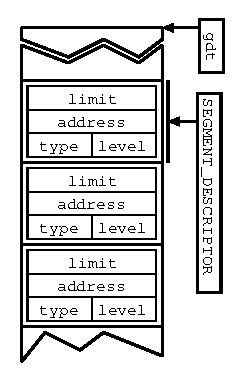
\includegraphics[scale=0.8]{figures/gdt.eps}
\end{column}
\end{columns}
\begin{alltt}
\ldots\\
~~\textcolor{red}{-}
\textcolor{blue}{gdt}:\textcolor{type}{NATIVE\_ARRAY}
(\textcolor{red}{Expanded} \textcolor{type}{SEGMENT\_DESCRIPTOR});\\
\end{alltt}
\end{block}

\end{frame}
%---------------------------------------------------
\begin{frame}{Memory Mapping\,: binary file structure (2/3)}
\begin{alltt}
\textcolor{red}{Section Header}\\
~~\textcolor{red}{+} \textcolor{blue}{name} := \textcolor{type}{MY\_STRUCT};\\
\textcolor{red}{Section Mapping}\\
~~\textcolor{red}{+} \textcolor{blue}{coord\_x}:\textcolor{type}{UINTEGER\_32};\\
~~\textcolor{red}{+} \textcolor{blue}{coord\_y}:\textcolor{type}{UINTEGER\_32};\\
~~\textcolor{red}{+} \textcolor{blue}{flags}:\textcolor{type}{UINTEGER\_16};\\
~~\textcolor{red}{+} \textcolor{blue}{color}:\textcolor{type}{UINTEGER\_16};\\
\textcolor{red}{Section Public}\\
~~\textcolor{red}{-} \textcolor{blue}{move} $\leftarrow$ \ldots\\
~~\textcolor{red}{-} \textcolor{blue}{set\_color} $\leftarrow$ \ldots\\
\end{alltt}
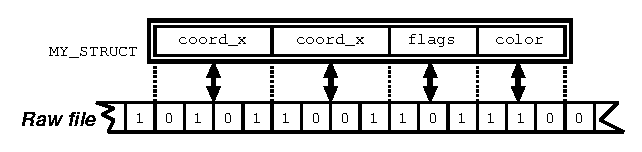
\includegraphics[scale=0.75]{figures/binary_struct.eps}
\end{frame}
%---------------------------------------------------
\begin{frame}{Memory Mapping\,: composite structure example (3/3)}
\begin{columns}
\begin{column}[l]{5.5cm}
\begin{alltt}
\textcolor{red}{Section Header}\\
~~\textcolor{red}{+} \textcolor{blue}{name} := \textcolor{type}{STRUCT\_1};\\
\textcolor{red}{Section Mapping}\\
~~\textcolor{red}{+} \textcolor{blue}{code}:\textcolor{type}{UINTEGER\_32};\\
~~\textcolor{red}{+} \textcolor{blue}{stat}:\textcolor{red}{Expanded} \textcolor{type}{STRUCT\_2};\\
~~\textcolor{red}{+} \textcolor{blue}{type}:\textcolor{type}{UINTEGER\_16};\\
\ldots\\
\textcolor{red}{Section Header}\\
~~\textcolor{red}{+} \textcolor{blue}{name} := \textcolor{type}{STRUCT\_2};\\
\textcolor{red}{Section Mapping}\\
~~\textcolor{red}{+} \textcolor{blue}{data\_1}:\textcolor{type}{UINTEGER\_16};\\
~~\textcolor{red}{+} \textcolor{blue}{data\_2}:\textcolor{type}{UINTEGER\_16};\\
\end{alltt}
\end{column}
\begin{column}[r]{4cm}
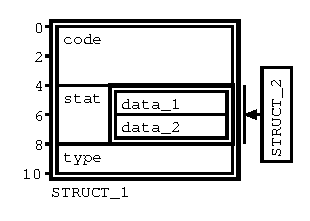
\includegraphics[scale=1.0]{figures/mapping_composite.eps}
\end{column}
\end{columns}
\end{frame}
%---------------------------------------------------
\begin{frame}{Interrupt hardware manager}
\begin{block}{Example}
\begin{alltt}
\textcolor{red}{Section Interrupt}\\
~~\textcolor{red}{-} \textcolor{blue}{my\_interrupt} $\leftarrow$\\
~~( // {\it{}Code Lisaac \ldots}\\
~~);
\end{alltt}
\end{block}
\begin{exampleblock}{Note}
\begin{itemize}
\item Can't a call direct \textcolor{blue}{my\_interrupt} slot
\item \textcolor{blue}{my\_interrupt} call send a
  \textcolor{type}{POINTER} address function. It's necessary for to
  put this address in Interrupt Descriptor Table.
\end{itemize}
\end{exampleblock}
\begin{alertblock}{Restriction}
\begin{itemize}
\item Parameter or result is prohibited
\item The function should not be Self dependent
\end{itemize}
\end{alertblock}
\end{frame}
%---------------------------------------------------
\begin{frame}{External C to Lisaac (1/4)}
\begin{block}{Example without result}
\begin{alltt}
\textcolor{red}{-} \textcolor{blue}{die\_with\_code}
code:\textcolor{type}{INTEGER} $\leftarrow$ \textcolor{red}{`exit(@code)`};
\end{alltt}
\end{block}
\begin{exampleblock}{Note}
\begin{itemize}
\item \textcolor{red}{\tt{}@<identifier>} for access to {\bf{}local variable only}\\
  (or argument)
\item This access is always {\bf{}read only}.
\end{itemize}
\end{exampleblock}
\end{frame}
%---------------------------------------------------
\begin{frame}{External C to Lisaac\,: with result (2/4)}
\begin{block}{Example}
\begin{itemize}
\item Persistant external\,:
  \begin{alltt}
\textcolor{red}{-} \textcolor{blue}{basic\_getc} $\leftarrow$
\textcolor{red}{`getchar()`}:(\textcolor{type}{CHARACTER});
  \end{alltt}
\item Non persistant external\,:
  \begin{alltt}
\textcolor{red}{- Self}:\textcolor{type}{SELF} \textcolor{blue}{'>>'} other:\textcolor{type}{SELF} :\textcolor{type}{SELF} $\leftarrow$
\textcolor{red}{`@Self>>@other`}:\textcolor{type}{SELF};
  \end{alltt}
\end{itemize}
\end{block}
\begin{exampleblock}{Note\,: Warning}
\begin{itemize}
\item {\bf{}Persistant}\,: The persistant external means that the code will
remain present even if the return value is not used. Parentheses in
the type of return shows that the return value is not important, is the
execution of this external is important.
\item {\bf{}Non persistant}\,:
If the result external is not used, then the
external is deleted by the compiler.
\end{itemize}
\end{exampleblock}
\end{frame}
%---------------------------------------------------
\begin{frame}{External C to Lisaac\,: dynamic type (3/4)}
\begin{block}{Example}
\begin{alltt}
\textcolor{red}{- Self}:\textcolor{type}{SELF} \textcolor{blue}{'>'} other:\textcolor{type}{SELF} :\textcolor{type}{BOOLEAN} $\leftarrow$
\textcolor{red}{`@Self>@other`}:\textcolor{type}{BOOLEAN}\{\textcolor{type}{TRUE},\textcolor{type}{FALSE}\};
\end{alltt}
\end{block}
\begin{exampleblock}{Note}
\begin{itemize}
\item This {\bf{}static type} result is \textcolor{type}{\tt{}BOOLEAN}
\item The {\bf{}dynamic type set} for this result is
  \textcolor{type}{\tt{}TRUE} or \textcolor{type}{\tt{}FALSE}
\item Each dynamic type must be a sub type of static type
\end{itemize}
\end{exampleblock}
\end{frame}
%---------------------------------------------------
\begin{frame}{External C to Lisaac\,: mapping C type (4/4)}
\begin{block}{Example}
\begin{alltt}
\textcolor{red}{Section Header}\\
~~\textcolor{red}{+} \textcolor{blue}{name} := \textcolor{red}{Expanded} \textcolor{type}{CHARACTER};\\
~~\textcolor{red}{-} \textcolor{blue}{type} := \textcolor{red}{`signed char`};
\end{alltt}
\end{block}
\begin{exampleblock}{Note}
The compiler translate the \textcolor{type}{\tt{}CHARACTER}
  with C type \textcolor{blue}{\tt{}signed char}
\end{exampleblock}
\begin{alertblock}{Warning}
With {\tt{}Expanded} or not and the C type\,:
\begin{itemize}
\item {\tt{}Expanded} type $\Longrightarrow$ No pointer C type
\item No {\tt{}Expanded} type $\Longrightarrow$ Pointer C type
\end{itemize}
\end{alertblock}

\end{frame}
%---------------------------------------------------
\begin{frame}{External Lisaac to C}

\begin{block}{examples}
\begin{alltt}
\textcolor{red}{Section External}\\
~~\textcolor{red}{-} \textcolor{blue}{function\_for\_c} (a,b:\textcolor{type}{INTEGER}) :\textcolor{type}{INTEGER} $\leftarrow$\\
~~( // {\it{}Code Lisaac \ldots}\\
~~);
\end{alltt}
\end{block}
\begin{exampleblock}{Note}
Here, we have a function \textcolor{blue}{\tt{}int function\_for\_c(int a,int b)} in C code product
\end{exampleblock}
\begin{alertblock}{Restriction}
\begin{itemize}
\item Several keywords for the name function is prohibited
\item The function should not be Self dependent
\item The vector result is prohibited
\end{itemize}
\end{alertblock}
\end{frame}
%---------------------------------------------------
\begin{frame}{External intern of Lisaac}
\begin{block}{Definition}
This is a fondamental external known and used by the compiler.\\
Syntax\,: \textcolor{red}{\tt{}`<number>`} with $number \in [0..31]$
\end{block}
\begin{block}{examples}
\begin{alltt}
\textcolor{red}{- Self}:\textcolor{type}{SELF} \textcolor{blue}{'-'} \textcolor{red}{Left 80} other:\textcolor{type}{SELF} :\textcolor{type}{SELF} $\leftarrow$ \textcolor{red}{`1`};\\
\textcolor{red}{- Self}:\textcolor{type}{SELF} \textcolor{blue}{'*'} \textcolor{red}{Left 100} other:\textcolor{type}{SELF} :\textcolor{type}{SELF} $\leftarrow$ \textcolor{red}{`2`};\\
\textcolor{red}{- Self}:\textcolor{type}{SELF} \textcolor{blue}{'/'} \textcolor{red}{Left 100} other:\textcolor{type}{SELF} :\textcolor{type}{SELF} $\leftarrow$ \textcolor{red}{`3`};\\
\textcolor{red}{- Self}:\textcolor{type}{SELF} \textcolor{blue}{'\&'} \textcolor{red}{Left 100} other:\textcolor{type}{SELF} :\textcolor{type}{SELF} $\leftarrow$ \textcolor{red}{`4`};\\
\textcolor{red}{- Self}:\textcolor{type}{SELF} \textcolor{blue}{'>'} \textcolor{red}{Left 100} other:\textcolor{type}{SELF} :\textcolor{type}{BOOLEAN} $\leftarrow$ \textcolor{red}{`5`};\\
\end{alltt}
\end{block}
\end{frame}
%---------------------------------------------------
\begin{frame}{COP\,: Concurrent Object Prototypes (1/4)}
\begin{center}
\includegraphics{figures/cop-comm.ps}
\end{center}
\end{frame}
%---------------------------------------------------
\begin{frame}{COP\,: Concurrent Object Prototypes (2/4)}
\begin{center}
  \includegraphics[scale=0.65]{figures/cop-clone.ps}
\end{center}
\end{frame}

%---------------------------------------------------
\begin{frame}{COP\,: Concurrent Object Prototypes (3/4)}
\begin{center}
  \includegraphics{figures/cop-assign.ps}
\end{center}
\end{frame}
%---------------------------------------------------
\begin{frame}{COP\,: Concurrent Object Prototypes (4/4)}
\begin{center}
  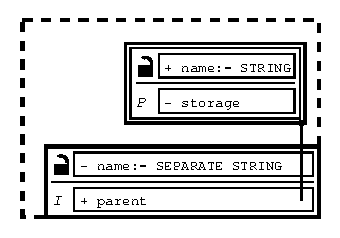
\includegraphics{figures/cop-separate.eps}
\end{center}
\end{frame}
%---------------------------------------------------
\section{Project manager}
%===============================
\begin{frame}{LIP\,: LIsaac Project manager (1/11)}

\includegraphics[scale=0.6]{figures/lip.eps} 
\begin{block}{One file = one project}
By default\,: {\tt{}lisaac/make.lip} 

\begin{itemize}
\item Communication between Compiler and Lip file\,:\\
{\it{}Via Intern variables}
\item Full configuration of compiler options
\item Subset Lisaac language Interpreter
\item Dynamic description of paths directories
\item Set of instructions before compilation pass (Front-end)
\item Set of instructions after compilation pass (Back-end)
\item Dynamic execution during compilation in live prototype context
\end{itemize}
\end{block}

\end{frame}
%---------------------------------------------------
\begin{frame}{LIP\,: Lip file location (2/11)}

\begin{block}{Explicite path for a Lip file}
\begin{alltt}
sonntag@isaac:$\sim$/slides/lisaac\$ {\bf{}lisaac ../project/make.lip}
\end{alltt}
\end{block}

\begin{block}{Implicite research}
\begin{enumerate}
\item Search lip file in current directory.
\item if failed, search in parent of directory.
\item go to (2) until the root directory
\item Else, search lip file by default ({\tt{}lisaac/make.lip})
\end{enumerate}
\end{block}

\end{frame}
%---------------------------------------------------
\begin{frame}{Lip\,: Intern variables (3/11)}

\begin{block}{Compiler $\Longrightarrow$ Lip {\it{}(immediately)}}
\begin{alltt}
  \textcolor{red}{+} \textcolor{blue}{lisaac}:\textcolor{type}{STRING};   
\end{alltt}
Example\,: {\tt{}/home/sonntag/lisaac/}
\begin{enumerate}
\item Read {\tt{}LISAAC\_DIRECTORY} environnement variable
\item if (1) failed, search {\tt{}\#define LISAAC\_DIRECTORY} in {\tt{}path.h}
\end{enumerate}
\end{block}

\begin{block}{Compiler $\Longrightarrow$ Lip {\it{}(immediately)}}
\begin{alltt}
  \textcolor{red}{+} \textcolor{blue}{input\_file}:\textcolor{type}{STRING};   
\end{alltt}
Example\,: {\tt{}hello\_world} {\it{}(Read command line argument)}
\end{block}

\begin{block}{Compiler $\Longrightarrow$ Lip {\it{}(after compilation)}}
\begin{alltt}
  \textcolor{red}{+} \textcolor{blue}{is\_cop}:\textcolor{type}{BOOLEAN};   
\end{alltt}
\end{block}

\end{frame}
%---------------------------------------------------
\begin{frame}{Lip\,: Intern variables (4/11)}

\begin{block}{Compiler $\Longleftarrow$ Lip {\it{}(Debug information)}}
\begin{alltt}
  \textcolor{red}{+} \textcolor{blue}{debug\_level}:\textcolor{type}{INTEGER};\\   
  \textcolor{red}{+} \textcolor{blue}{debug\_with\_code}:\textcolor{type}{BOOLEAN}; \\
  \textcolor{red}{+} \textcolor{blue}{is\_all\_warning}:\textcolor{type}{BOOLEAN};   
\end{alltt}
\end{block}

\begin{block}{Compiler $\Longleftarrow$ Lip {\it{}(Optimization)}}
\begin{alltt}
  \textcolor{red}{+} \textcolor{blue}{is\_optimization}:\textcolor{type}{BOOLEAN};\\   
  \textcolor{red}{+} \textcolor{blue}{inline\_level}:\textcolor{type}{INTEGER};   
\end{alltt}
\end{block}

\end{frame}
%---------------------------------------------------
\begin{frame}{Lip\,: Intern variables (5/11)}

\begin{block}{Compiler $\Longleftarrow$ Lip {\it{}(Generate code)}}
\begin{alltt}
  \textcolor{red}{+} \textcolor{blue}{is\_java}:\textcolor{type}{BOOLEAN};   
\end{alltt}
\end{block}

\begin{block}{Compiler $\Longleftarrow$ Lip {\it{}(Other)}}
\begin{alltt}
  \textcolor{red}{+} \textcolor{blue}{is\_statistic}:\textcolor{type}{BOOLEAN}; \\
  \textcolor{red}{+} \textcolor{blue}{is\_quiet}:\textcolor{type}{BOOLEAN};   
\end{alltt}
\end{block}

\end{frame}
%---------------------------------------------------
\begin{frame}{Lip\,: Subset Lisaac language (6/11)}

\begin{block}{Syntax}
\begin{itemize}
\item Types\,: \textcolor{type}{BOOLEAN, STRING, INTEGER}
\item Binary Operators\,: \textcolor{red}{
\begin{alltt}| ~~\& ~~$+$ ~~$-$ ~~$<$ ~~$>$ ~~$\le$ ~~$\ge$ ~~$=$ ~~$!=$
\end{alltt}
}
\item Unary Operators\,: \textcolor{red}{- ~~ !}
\item Assignment\,: \textcolor{red}{:=}
\item Style slot\,: 
  \begin{itemize}
  \item \textcolor{red}{\tt{}+} data slot
  \item \textcolor{red}{\tt{}-} method slot\\
        {\it{}(with 0 or 1 parameter and without return value)}
  \end{itemize}
\end{itemize}
\end{block}
\end{frame}
%---------------------------------------------------
\begin{frame}{Lip\,: Subset Lisaac language (7/11)}

\begin{block}{Slot built-in} 
\begin{itemize}
\item \textcolor{type}{BOOLEAN}.\textcolor{blue}{if} \textcolor{type}{\{ \ldots \}}
\item \textcolor{type}{BOOLEAN}.\textcolor{blue}{if} \textcolor{type}{\{ \ldots \}} \textcolor{blue}{else} \textcolor{type}{\{ \ldots \}}
\item \textcolor{type}{BOOLEAN}$\|$\textcolor{type}{STRING}$\|$\textcolor{type}{INTEGER}.\textcolor{blue}{print}
\item \textcolor{blue}{path} text:\textcolor{type}{STRING}
\item \textcolor{blue}{run} cmd:\textcolor{type}{STRING} :\textcolor{type}{INTEGER}
\item \textcolor{blue}{get\_integer}:\textcolor{type}{INTEGER}
\item \textcolor{blue}{get\_string}:\textcolor{type}{STRING}
\item \textcolor{blue}{exit}
\end{itemize}
\end{block}

\end{frame}
%---------------------------------------------------
\begin{frame}{Lip\,: Option description (8/11)}

\begin{block}{In \textcolor{red}{Section Public}} 
\begin{alltt}
\textcolor{red}{-} \textcolor{blue}{debug} level:\textcolor{type}{INTEGER} $<-$\\
\textcolor{red}{{\it{}// Fix debug level (default: 15)}}\\
(\\
~~((level $<$ 1) | (level $>$ 20)).\textcolor{blue}{if} \{\\
~~~~"Incorrect debug level.".\textcolor{blue}{print};\\
~~~~\textcolor{blue}{exit};\\
~~\};\\
~~\textcolor{blue}{debug\_level} := level;\\
);
\end{alltt}
\end{block}

\begin{block}{Compiler Lisaac option} 
\begin{alltt}
Options:\\
~~-debug <level:INTEGER> :\\
~~~~~~~~~Fix debug level (default: 15)\\
\end{alltt}
\end{block}
\end{frame}
%---------------------------------------------------
\begin{frame}{Lip\,: Other Section (9/11)}

\begin{block}{In \textcolor{red}{Section Private}} 
\begin{itemize}
\item Others code slots.
\item Data slot intern and others data slots.
\end{itemize}
\end{block}

\begin{block}{In \textcolor{red}{Section Inherit} {\it{}(Multi-inheritance)}} 
\begin{itemize}
\item With lip path\,:
\begin{alltt}
\textcolor{red}{+} \textcolor{blue}{parent}:\textcolor{type}{STRING} := ``../my\_project/linux/'';
\end{alltt}
\item Without path\,: Inheritance Lip file by default.
\begin{alltt}
\textcolor{red}{+} \textcolor{blue}{parent}:\textcolor{type}{STRING};
\end{alltt}
\end{itemize}
\end{block}

\begin{alertblock}{Inheritance}
\begin{itemize}
\item Redefinition slot is authorized.
\item Lookup algorithm is active.
\end{itemize}
\end{alertblock}

\end{frame}
%---------------------------------------------------
\begin{frame}{Lip\,: Particular method slot (10/11)}

\begin{block}{front\_end} 
Executed by compiler, before compilation step.
\begin{itemize}
\item Detect operating system,
\item Loading path set for a project,
\end{itemize}
\end{block}

\begin{block}{back\_end} 
Executed by compiler, after compilation step.
\begin{itemize}
\item Added {\tt{}gcc} options, lib, \ldots
\item Finalize the compilation with {\tt{}gcc} or others
\end{itemize}
\end{block}

\begin{alertblock}{Warning}
\textcolor{blue}{back\_end} \& \textcolor{blue}{front\_end} 
is mandatory in \textcolor{red}{Section Private}
\end{alertblock}

\end{frame}
%---------------------------------------------------
\begin{frame}{Lip\,: Dynamic execution during compilation (11/11)}

\begin{block}{In the \textcolor{red}{Section Header}} 
\begin{alltt}
\textcolor{red}{Section Header}\\
~~\textcolor{red}{+} \textcolor{blue}{name} := \textcolor{type}{VIDEO};\\
~~\textcolor{red}{-} \textcolor{blue}{lip} $<-$ ( \textcolor{blue}{add\_lib} ``-lX11''; );
\end{alltt}
\end{block}

\begin{block}{In {\tt{}make.lip}} 
\begin{alltt}
\textcolor{red}{-} \textcolor{blue}{add\_lib} lib:\textcolor{type}{STRING} $<-$\\
(~\textcolor{blue}{run} "echo $\backslash$"int main()\{ return(1); \}$\backslash$" $>$ \_t.c";\\
~~(\textcolor{blue}{run}("gcc \_t.c"$+$lib$+$" 2$>$/dev/null")$=$0).\textcolor{blue}{if} \{\\
~~~~\textcolor{blue}{lib\_gcc} := \textcolor{blue}{lib\_gcc} $+$ " " $+$ lib;\\
~~\} \textcolor{blue}{else} \{\\
~~~~("ERROR: `" $+$ lib $+$ "' lib not found.").\textcolor{blue}{print};\\
~~~~\textcolor{blue}{run} "rm \_t.c";~~\textcolor{blue}{exit};\\
~~\};\\
);
\end{alltt}
\end{block}
\end{frame}
%---------------------------------------------------
\section{Conclusion}
%===============================
\begin{frame}{Question ?}
\begin{block}{IRC}
\begin{itemize}
\item Server: {\tt{}irc.oftc.net}
\item Channel: {\tt{}\#isaac}
\end{itemize}
\end{block}

\begin{block}{Information \& contacts}
\begin{itemize}
\item {\bf{}Wiki}\,: {\tt{}http://wiki.lisaac.org}
\item {\bf{}Mailing list}\,: {\tt{}http://www.lisaac.org/community/contact}
\end{itemize}
\end{block}
\begin{center}

\includegraphics[scale=0.5]{figures/isaac_logo.eps} 
\end{center}
\begin{flushright}
{\it{}Good luck!}
\end{flushright}
\end{frame}


\end{document}
